\documentclass[10pt]{article}
\usepackage{amsmath}
\usepackage{commath}
\usepackage{algorithm}
\usepackage{algorithmic}
\usepackage{url}
\usepackage{cite}
\usepackage{amsfonts}
\usepackage{footnote}
\usepackage{footmisc}
\usepackage{enumitem}
\usepackage{todonotes}
\usepackage{graphicx}
\graphicspath{{./images/}}

\begin{document}

\title{Applied and Computational Mathematics Master's Thesis Semester Report}
\author{Erick Galinkin}
\maketitle

\section{Introduction}
Malicious software (malware), has long been a burden on users of computers and of  the internet.
For individuals, a malware attack can cause the loss of their personal data and may allow hackers to access their bank accounts, steal their identity, or hold all of the files on their computer ransom.
The effects for a business can be particularly dire, with average cost of a malware attack sitting at \$1.7 million~\cite{seals2019threatlist}.
This problem is continuing to grow, and malware authors innovate in an effort to circumvent existing mitigating controls.

In the case of mobile malware, we often do not have the luxury of running computationally intensive processes on an endpoint and often cannot restrict devices that are brought into our environment.
 Traditional intrusion detection systems like Snort continue to mitigate known threats, but these signature-based systems suffer from the curse of reactivity for unknown threats.
 In order to mitigate these threats, controls must be generic enough to block threats which are unknown over any channel.

Our key contribution is an analysis of the impact Fourier and wavelet transforms have on unprocessed data as it relates to neural networks. 
This is achieved through an analysis of the efficiency and accuracy of a neural network that can detect the presence of malware on a mobile device without the need for an agent on the endpoint.
We compare this to a baseline random forest result and seek to explain what the network has learned and why different networks performance varies.

At the present time, the results may be divided into two categories:
\begin{enumerate}
\item Results on the augmented data associated with Watkins \textit{et al.}~\cite{watkins2018network} which suggest that a decision tree or other statistical learning method may be superior to a neural network and are explained below in section \ref{malware classifier}.
\item Analysis of how the representation of the data impacts the accuracy of a neural network and are explained in section \ref{data representation}
\end{enumerate}

\section{Previous Research}
The most significantly related previous research was conducted by Watkins \textit{et al.}~\cite{watkins2018network}.
This research yielded detections of mobile malware as the result of ping delays caused by CPU throttling in Android phones and an augmented version of their data set forms the basis for our research.
In the Watkins literature, a decision tree algorithm within the WEKA package was used to classify the traffic.
Similarly, we use a random forest from the Scikit-learn~\cite{scikit-learn} Python package as a baseline model.

Deep neural networks have been applied to related problems in information security, particularly detecting malicious executables on endpoints~\cite{raff2018malware} using techniques from natural language processing and computer vision.
This research, conducted at Nvidia labs worked well at the endpoint, examining static properties of malicious and benign executables to draw determinations about the software from byte sequences.

The use of Fourier transforms in neural networks has been of interest for some time and there are several papers on the subject~\cite{osowski2002fourier, pratt2017fcnn, highlander2016very} which consider these applications.
We lean most heavily on the paper by Pratt \textit{et al.}~\cite{pratt2017fcnn} due to its recency and implementation details. 
Particularly, this paper considers the impact of the convolution theorem within neural networks and uses the Fast Fourier Transform to quickly compute $\mathcal{F}(\kappa * u) = \mathcal{F}(\kappa) \odot \mathcal{F}(u)$ where $\mathcal{F}$ is the Fast Fourier Transform, $*$ denotes convolution, and $\odot$ denotes the Hadamard Pointwise Product.
This method is much faster since it requires significantly fewer computational operations than the more traditional sliding kernel method.
They also describe a Fourier Pooling Layer to reduce the data size while retaining information by truncating the boundaries of the matrices.
Ultimately, the paper shows that on the CIFAR-10 and MNIST datasets, the overall accuracy is lower than benchmark results - though the network trains and evaluates images much more quickly.

Wavelet neural networks pioneered by Fujieda \textit{et al.}~\cite{fujieda2017wavelet} have shown promise for generalized pooling and convolution by abstracting them into downsampling and filtering in the spectral domain.
The results in the Fujieda paper were significant, as the network achieved better accuracy results than AlexNet on the target dataset while having approximately 1/4 the number of parameters.
In addition, the memory requirements and speed of the network were a significant improvement on the other architectures considered by Fujieda.
It is worth noting that implementation details for the paper are sparse, and so our implementation may differ from this reference implementation. 

\section{Android App Data}
The data were collected from 123 free Android apps downloaded from the Google Play store. 
Of these apps, 68 were classified benign and 55 were classified malicious.
The specific methods for collecting the data and classifying the samples is detailed in Watkins \textit{et al.}~\cite{watkins2018network}
Two datasets were examined for the classifier: these were ``request-reply'' data, and ``reply-reply'' data.
The request-reply data is the latency between a ping request being sent and a reply being received - 100 of these measurements were collected per sample.
The reply-reply data is quite similar except that the data measured the latency between a reply and a subsequent reply.
% In the final report, we likely want to spell out the Fourier Transform and the continuous wavelet transform.
% That will probably be its own section, maybe an appendix? 

In addition to these two raw datasets, we also examined the Fourier transform of the datasets and a wavelet transform of the datasets. 
Given the large number of wavelets that exist, we chose the Morlet wavelet as the mother wavelet for the data transform due to how friendly it was with the data and the fact that it is uniquely invertible.
It is also noteworthy that due to the difficulty in inverting a continuous wavelet transform (See Appendix~\ref{inverse cwt}), a different wavelet - namely, the Haar Wavelet - was chosen for the wavelet neural network described in section \ref{wavelet cnn}.

Summary statistics for the aforementioned 6 datasets are in Table~\ref{Tab:summary}. 
For the non-raw datasets, only the first word of the transformed dataset is included (\textit{e.g.}, Fourier Transformed Request-Reply becomes ``Fourier Request'')

\subsection{Analysis}
One interesting effect of performing the transforms on the dataset is that while the continuous wavelet transform reduces our variance significantly and slightly normalizes the dataset, the Fourier transform has the opposite effect, introducing tremendous amounts of noise into the dataset.
As we discuss in section~\ref{data representation}, this likely has a meaningful impact on how much the network can learn, and may also explain some of the results found by Pratt \textit{et al.}~\cite{pratt2017fcnn}.

\renewcommand{\thefootnote}{*} 
\begin{table}[h]
\caption{Dataset Summary Statistics}
\centering
\label{Tab:summary}	
\begin{tabular}{l|llll}
\textbf{Dataset Name} & \textbf{Mean} & \textbf{Median} & \textbf{Mean Var.} & \textbf{Median Var.} \\\cline{1-5}
Request-Reply         & 27.43    & 10.07    & 8329.96    & 7663.89 \\
Reply-Reply           & 98.52    & 100.93   & 2688.85    & 2465.29 \\
Fourier Request       & 58.60\footnotemark    & -1.45    & 12229005.34    & 7418186.12 \\
Fourier Reply         & 100.19\footnotemark    & -6.82    & 119373138.03    & 122613924.30 \\
Wavelet Request       & 1.30    & -.072    & 1887.5    & 1507.16 \\
Wavelet Reply         & 1.03    & 0.12    & 2224.56    & 2135.86                 
\end{tabular}
\end{table}
\footnotetext{There is an extremely small, but non-zero imaginary part, on the order of $10^{-19}i$}

\renewcommand{\thefootnote}{1}

\section{Models}
All code\footnote{Code is available at the following url: \url{https://github.com/erickgalinkin/jhu_masters}} was written in Python, using the Tensorflow 2.0, PyTorch, and Scikit-learn libraries.
Only the baseline models described in \ref{other models} used the Scikit-learn library, and only the Wavelet Convolutional network described in \ref{wavelet cnn} used PyTorch.
The remaining models all used the Tensorflow framework.
All models were trained and tested on a 2018 MacBook Pro with 32GB of RAM and a 2.9GHz Intel Core i9 processor.
Given the small size of the data and relative simplicity of the models, GPU acceleration was not needed.
The sections here describe only the details of the architecture.
An overview of the machine learning algorithms is provided in appendix~\ref{ml algo}, and a more thorough treatment is available in Hastie~\cite{hastie01statisticallearning} or James~\cite{james14introduction}

\subsection{Standard Fully-Connected Neural Network}
The fully-connected neural network architecture accepts, as input, a 1x100 row-vector. 
This vector is then fed to three densely connected layers, each with 256 ReLU-activated neurons.
The output neuron is a single sigmoid-activated neuron, which provides a probability of traffic being benign.

\subsection{Standard Convolutional Neural Network}
Our standard convolutional neural network is a sequential model which accepts the same sort of input as our fully-connected neural network, and passes it to an architecture comprised of two convolution and max-pooling blocks, followed by batch normalization, and then passed to two densely connected layers of 128 neurons each. The architecture is visualized below in figure \ref{fig:conv net}.

\begin{figure}[ht]
\caption{Standard Convolutional Neural Network Architecture}
\label{fig:conv net}
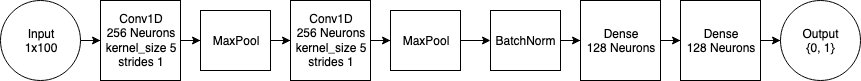
\includegraphics[width=\textwidth]{conv_architecture}
\centering
\end{figure}

\subsection{Fourier Convolutional Neural Network}
The Fourier Convolutional Neural Network leverages a custom "Fourier Layer", which moves the data into Fourier space via the Fast Fourier Transform before it performs a dot product on the input to the neuron.
Specifically, given an input $X^{(n)}$ and an output $A$, where the superscript is not an exponent, but instead indicates the layer of the input, the Fourier layer, $\ell$ acts on $X$: 
\begin{align*}
X^{(n+1)} & = a \\
& = \ell^{(n)}(X^{(n)}) \\
& = \sigma(\mathcal{F}^{-1}(\mathcal{F}(X^{(n)})\cdot \mathbf{W}^{(n)\top}))
\end{align*}

Where $\mathcal{F}$ is the Fast Fourier Transform, $\sigma$ is the activation function - ReLU in this case - and $\mathbf{W}$ is the weight matrix for layer n.

\begin{algorithm}
\caption{Fourier Layer}
\label{Fourier layer}
\begin{algorithmic}[1]
\REQUIRE $X, W \in \mathbb{C}^{mxn}, \beta \in \mathbb{C}^m$
\ENSURE $X \neq 0$
\STATE Perform Fourier transform on input data: $\mathcal{F}(X^{(n)})$
\STATE Take dot product of input data and weight matrix: $\mathcal{F}(X^{(n)})\cdot \mathbf{W}^{(n)\top}$
\STATE Perform Inverse Fourier transform on the dot product: $\mathcal{F}(\mathcal{F}(X^{(n)})\cdot \mathbf{W}^{(n)\top})$
\STATE Apply ReLU activation: $a = \sigma(\mathcal{F}^{-1}(\mathcal{F}(X^{(n)})\cdot \mathbf{W}^{(n)\top}))$
\STATE Return $a$
\end{algorithmic}
\end{algorithm}

Our Fourier ``Convolutional'' neural network is a mirror image of our standard convolutional neural network, only with the convolutional layers replaced by Fourier layers.
Here, we put the word convolutional in scare quotes due to the fact that no actual convolution is performed and thus it is a misnomer.
To be more intellectually honest, we should refer to this network instead as a ``Fourier Transform Inner Product Network'', though this may confuse readers unfamiliar with the relationship.
In the interest of broad understanding, the term convolutional neural network is used when it helps elucidate meaning even in spite of being a slight misnomer.

\subsection{Wavelet Convolutional Neural Network} \label{wavelet cnn}
The Wavelet Convolutional Neural Network implements similar functionality to our Fourier Neural Network, using the Continuous Wavelet Transform in lieu of the Fourier transform.
Due to the fact that there is a time component and a frequency component, the wavelet neural network has a higher dimensionality than our other models. 



\subsection{Other Models} \label{other models}
Two baseline models were considered.
The first is the random forest model provided in the Scikit-learn library with no hyperparameter tuning.
Decision tree models are generally good at classification tasks~\cite{hastie01statisticallearning} but are weak classifiers which are sensitive to variance.
Random forests are a the result of averaging a large collection of de-correlated trees and provide a good benchmark as a na\"ive model - in the respect that it is untuned - for classification.

The other benchmark model is a Support Vector Classifier, again provided by the Scikit-learn library.
The rationale for using a Support Vector Machine is that we wanted to see if some hyperplane could be learned which would separate the data.
This model was again, na\"ive in the respect that it was merely the ``out of the box'' model, and so the classifier was built on top of the radial basis function kernel.

\section{Results}
Here, our results are divided into two sections. 
The first considers the efficacy of the malware classifier and where certain improvements could be made.
The second section considers how the internal and external representation of our datasets influenced the ability of the neural network to learn.

\subsection{Malware Classifier} \label{malware classifier}
As shown in Table~\ref{Tab:test}, the Random forest classifier outperforms all of the neural network and support vector machine architectures.
It is also noteworthy that the Fourier-transformed data fed to the convolutional Neural Network appears to misclassify an extremely high percentage of samples, and by flipping the labels on the test samples, we actually achieve 72.6\% accuracy, making it our second most accurate neural network classifier.

 
\begin{table}[h]
\caption{Android App Data Test Results}
\centering
\label{Tab:test}	
\begin{tabular}{lll}
Data and Architecture Combination & Test Accuracy & mean step time (ms) \\
Raw, Fully-Connected NN           & 62.60\%         & 13                  \\
Raw, Convolutional NN             & 72.89\%         & 54                  \\
Fourier, Fully-Connected NN       & 55.28\%       & 12                  \\
Fourier, Convolutional NN         & 27.40\%         & 56                  \\
Wavelet, Fully-Connected NN       & 61.95\%         & 12                  \\
Wavelet, Convolutional NN         & 70.77\%         & 52                  \\
Raw, Fourier NN                   & 66.59\%         & 553                 \\
Raw, Wavelet NN                   & 00.00\%*        & 000*                \\
Raw, Random Forest                & 79.80\%         & N/A                 \\
Raw, Support Vector Classifier    & 55.28\%         & N/A                
\end{tabular}
\end{table}
 
\subsection{Data Representation and Neural Networks} \label{data representation}
aaaa

\section{Conclusions and Ongoing Work}
Overall, the results are interesting, even if they do not immediately improve on the state-of-the-art. 
Neural networks are well-understood to be data-intensive, and the scale of data associated with the Android App Dataset is likely not sufficiently large for a neural network to appropriately converge. 
The convolutional neural network approaches the performance of the untuned random forest algorithm but does not achieve the same level of accuracy.
Additionally, the random forest algorithm is much faster to train, and requires no advanced hyperparameter tuning.
We will continue to make improvements to the networks and also test our architectures on different datasets, as explained below.

Based on the difficulty and apparent inefficiency on small datasets of the Fourier and Wavelet neural networks, alternate activation functions are being considered. 
However, finding good spectral activation functions is still an open research question.
In their paper on deep complex networks, Trabelsi \textit{et al.}~\cite{trabelsi2017deep} use the Complex ReLU ($\mathbb{C}$Relu) and so-called $z$ReLU functions. 
Neither of these have yet been tried on the complex-valued data in the Fourier or Wavelet neural networks.

Pennec and Arsigny~\cite{pennec2013information} suggest that in high dimensional spaces, we can view our data as a manifold and thereby consider the Riemannian center of mass or \textit{Frechet mean} of the manifold.
Further research by Chakraborty \textit{et al.}~\cite{chakraborty2019surreal} suggests that in manifold-valued data, the possibility of using the tangent-ReLU activation function may make it feasible to move the data to and from the Fourier domain only once per pass through the network, instead of once per layer.
At this point, none of these techniques have been implemented in code, and our data may be too simple to fully validate the efficacy of these techniques.

In order to remedy some of the hurdles of this dataset, we also plan to try these on computer vision tasks, specifically the CIFAR-10~\cite{krizhevsky2009learning} dataset, as it will provide a higher dimensional dataset. 
By using more traditional benchmarks, we can also better contextualize our results here, and how the Fourier and Wavelet networks perform on these tasks.
This work will likely be time consuming, but is still feasible within our time constraints.

Although there is significant ongoing work, the bulk of the research allows us to conclude that for this dataset, the best classifier is likely some kind of decision tree.
It may be fruitful to find a well-tuned decision tree classifier, pair it with the script which generated the data, and treat those results separately as a conference or journal paper. 
That decision remains to be made at the time of this writing.

\bibliography{bibtex}
\bibliographystyle{siam}

\appendix
\section{Description of Machine Learning Algorithms}\label{ml algo}
asdfasdfasdf
\end{document}
